\appendix
\chapter{Example Tree of Some $\mathcal{Q}$}
\label{app:tree}
\centering
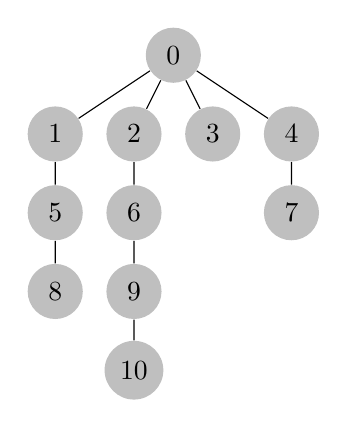
\begin{tikzpicture}[level/.style={sibling distance=10mm/#1, level distance=10mm}]
\tikzset{every node/.style={shape=circle,fill=black!25,minimum size=7mm}}
%\tikzset{every node/.style={shape=circle,
%                            font=\bfseries \Large,
%                            minimum size=3cm,
%                            scale=0.4
%                           }}
\node (root) {$0$}
    child {
        node {$1$}
        child {
            node (n5) {$5$}
            child {
                node {$8$}
            }
        }
    }
    child {node (n2) {$2$}
        child {node (n6) {$6$}
            child {node {$9$}
                child {node {$10$}
                }
            }
        }
    }
    child {node (n3) {$3$}
    }
    child {node (n4) {$4$}
        child {node {$7$}
        }
    }
    ;
\end{tikzpicture}


\chapter{Slp Header Files}

\section*{\texttt{Algorithm.hpp}}
\begin{verbatim}
/**
 * Perform a line search by finding the minimum objective value
 * of the given QP problem of all the points between the two
 * given points.
 *
 * @param  p1
 *         Start point.
 * @param  p2
 *         End point.
 * @param  model
 *         ClpModel of the QP problem.
 * @return the step length alpha.
 */
double lineSearch(double* p1, double* p2, const ClpModel model);
\end{verbatim}

\begin{verbatim}
/**
 * Solve a QP problem using Slp.
 *
 * @param  quad
 *         ClpModel containing the QP problem.
 * @param  x
 *         Array containing the initial guess vector. This array
 *         will be overwritten with a final solution.
 * @param  maxIters
 *         Number of iterations to perform if the stopping
 *         criteria is not met.
 * @param  tol
 *         Epsilon for the stopping criteria.
 * @return the objective value of the solved QP problem..
 */
double solve(ClpModel quad, double* x, int maxIters, double tol);
\end{verbatim}

\newpage

\begin{verbatim}
/**
 * Perform a Taylor-series expansion of the objective function of
 * the given QP problem at the given point.
 *
 * @param destCoeffs
 *        Pointer to coefficient destination.
 * @param point
 *        Point to perform the expansion at.
 * @param model
 *        ClpModel that has the objective function.
 */
void taylor(double* destCoeffs, double* point, ClpModel model);
\end{verbatim}

\begin{verbatim}
/**
 * Evaluate the objective function of the given model at
 * the given point.
 *
 * @param point
 *        Point to evaluate the objective function at.
 * @param model
 *        ClpModel that has the objective function to evaluate.
 */
doubld value(double* point, ClpModel model);
\end{verbatim}
